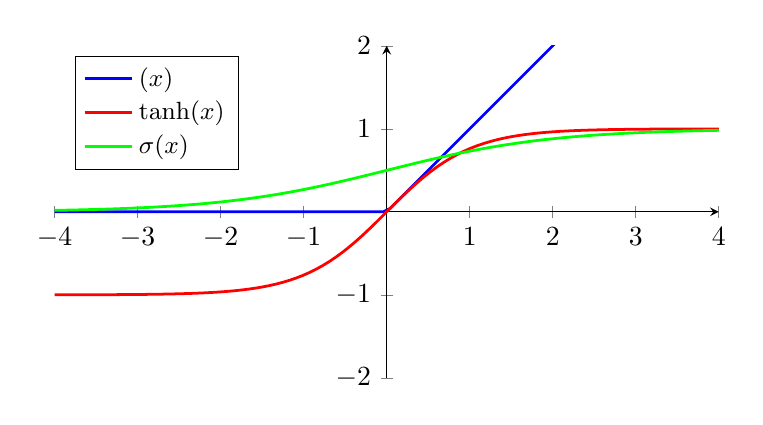
\begin{tikzpicture}
    \begin{axis}[
        axis lines = left,
        y=30,
        x=30,
        ymin = -2, ymax = 2,
        xmin = -4, xmax = 4,
        axis lines=middle,
        legend pos={north west},
        legend cell align={left},
        legend style={font=\small},
    ]

    \addplot [
        domain=-4:4, 
        samples=100, 
        color=blue,
        line width=1pt
    ]
    {(x + abs(x)) / 2};
    \addlegendentry{$\relu(x)$};
    
    \addplot [
        domain=-4:4, 
        samples=100, 
        color=red,
        line width=1pt
    ]
    {tanh(x)};
    \addlegendentry{$\tanh(x)$};

    \addplot [
        domain=-4:4, 
        samples=100, 
        color=green,
        line width=1pt
    ]
    {e^x / (1 + e^x)};
    \addlegendentry{$\sigma(x)$}
    \end{axis}
\end{tikzpicture}
